\chapter{Physics of lepton colliders}
\label{Lepton_Physics}
\begin{chapterabstract}
The physics done at particle colliders, where two particle beams are brought into collision, is the physics of atoms and quanta, of nuclei and partons, of particles that build up everything we know, but also of new particles, physics beyond our current knowledge.
After a brief introduction of the Standard Model, a theory describing the elementary particles and the fundamental forces, the physics processes at a lepton collider will be explained in more detail.
\end{chapterabstract}
\newline

Particle physics reaches back to the ancient Greek times, when the idea was developed that matter is made of ``indivisible'' (\'atomos, Greek) parts.
Atoms are, in fact, not indivisible at all.
When the electron was experimentally discovered in 1897 by J.J. Thomson, it was proposed that these particles must be a component of every atom.
That sparked the interest of many physicists in the early \nth{20} century to perform experiments probing atoms.
One of them was Ernest Rutherford, who fired alpha particles\footnote{An alpha particle is the nuclei of a Helium atom. Ernest Rutherford obtained them from radioactive decays of uranium amongst others.} through a thin gold foil, and thereby found that atoms are mostly empty with a positively charged nucleus that is about 3000 times smaller\footnote{From more precise measurements that are possible nowadays, the nucleus of hydrogen for example is, in fact, about \num{33000} times smaller than the hydrogen atom.} than the atom.
This discovery was a crucial step towards the modern atomic model.\\
Close to our current understanding of the atomic model is the Bohr model, developed by Niels Bohr in 1913.
It describes that electrons orbit the positively charged nucleus on stable shells with distinct radii.
The shells correspond to discrete energies, such that an electron switching from one shell to a shell with a larger radius would have to absorb energy, or emit energy respectively.
This energy quantum is absorbed or emitted in form of light, more precisely in form of a photon.
Nowadays, it is known that the electrons do not orbit the nucleus on discrete shells but rather in orbital zones, where the electron has a higher probability to be observed.\\
In order for an atom to have a neutral charge, the number of electrons in the atomic shells have to be balanced by an equal amount of positive charge of the nucleus.
That nuclei of different atoms are built from the hydrogen nucleus was already proven by Rutherford in 1917.
He thereby discovered the proton, and explained that the positive charge of the nucleus is the summed up charges of the protons inside the nucleus.\\
In 1932, it was found that atoms can not only consist of electrons and protons.
The mass measurements of various isotopes showed that their masses differ by concrete amounts.
The explanation was that the nucleus must consists of protons and particles with a similar mass but a neutral charge, the neutrons.
Isotopes are therefore atoms of the same element with the same number of protons, but with a different amount of neutrons.\\
The development of particle accelerators that can accelerate particles to higher and higher energies allowed to probe even the constituents of the atom.
This showed that the end has not been reached yet, that protons and neutrons are not elementary but composite particles.
Their partons, the so-called quarks, are part of the current theory of all elementary particles and the fundamental forces they interact with, the Standard Model.
\section{The Standard Model}
\label{StandardModel}
The Standard Model explains how the elementary particles interact with each other via the fundamental forces of the universe.

\section{Production modes}
\label{Production_modes}
\section{Backgrounds}
\label{Backgrounds}
\subsection{High cross-section backgrounds from beam-beam interactions}
\label{BeamBeam}
\subsubsection{Pair background}
\label{BeamBeam:pairs}

\begin{figure}
\begin{subfigure}[b]{0.33\textwidth}
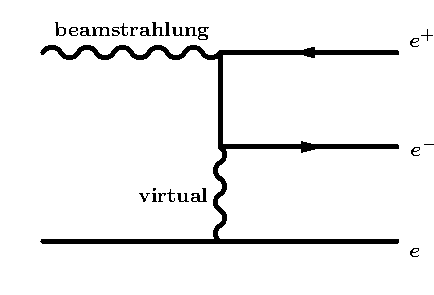
\includegraphics[width=\textwidth]{Figures/Bethe-Heitler.pdf}
\caption{Bethe-Heitler}
\end{subfigure}
\begin{subfigure}[b]{0.33\textwidth}
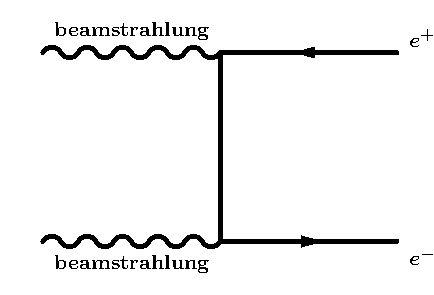
\includegraphics[width=\textwidth]{Figures/Breit-Wheeler.pdf}
\caption{Breit-Wheeler}
\end{subfigure}
\begin{subfigure}[b]{0.33\textwidth}
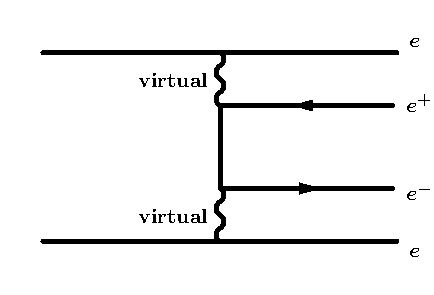
\includegraphics[width=\textwidth]{Figures/Landau-Lifshitz.pdf}
\caption{Landau-Lifschitz}
\end{subfigure}
\caption[LO Feynman diagrams of the production of the background pairs.]{The LO Feynman diagrams of the production processes of the background pairs: Bethe-Heitler, Breit-Wheeler and Landau-Lifschitz.}
\label{fig:Feynman:pair_production}
\end{figure}

\subsubsection{Bhabha scattering and $\gamma\gamma\rightarrow$hadrons}
\label{BeamBeam:bhabha_gammagamma}

\begin{figure}
\centering
\begin{subfigure}[b]{0.35\textwidth}
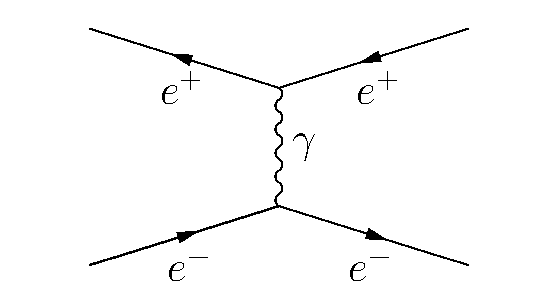
\includegraphics[width=\textwidth]{Figures/bhabha_scattering.pdf}
\caption{Bhabha scattering}
\end{subfigure}
\vspace*{0.2cm}
\begin{subfigure}[b]{0.35\textwidth}
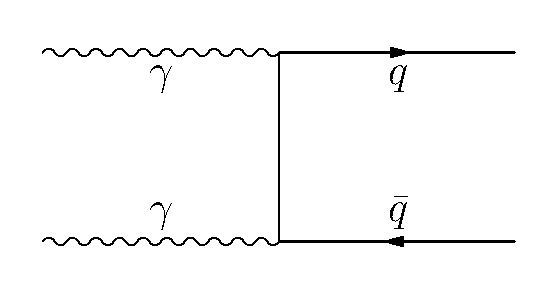
\includegraphics[width=\textwidth]{Figures/gammagamma_hadrons.pdf}
\caption{$\gamma\gamma\rightarrow$hadrons}
\end{subfigure}
\caption[LO Feynman diagrams of bhabha scattering and the $\gamma\gamma\rightarrow$hadrons process.]{The LO Feynman diagrams of the bhabha scattering and the $\gamma\gamma\rightarrow$hadrons process.}
\label{fig:Feynman:bhabha_gammagamma}
\end{figure}

\subsection{Machine backgrounds}
\label{MachineBackgrounds}